% Tableaux de résultats, graphiques
% Préciser l'erreur
% Incertitudes

Tout d'abord, la table ci-dessous présente les spécifications du fabricant du solénoïde, soit sur le nombre de spire et la longueur qui leur correspond.
Notons que c'est uniquement pour un des deux côtés, et que concrètement il y a deux fois plus de spire sur une longueur deux fois plus longues, mais sur la première approximation par la loi d'Ampère, cela ne change rien car ces facteurs se compensent, et sur la seconde cela se voit uniquement dans le calcul des angles.

\begin{table}[H]
\centering
\begin{tabular}{rr}
\toprule
 nombre de spires &  longueur $[mm]$ \\
\midrule
        5 &  10.3 \\
       10 &  20.6 \\
       20 &  40.3 \\
       30 &  60.9 \\
       50 & 101.2 \\
       70 & 141.6 \\
      100 & 202.5 \\
\bottomrule
\end{tabular}
\caption{Demi-longueur associée au demi-nombre de spires}
\end{table}

\paragraph*{Première expérience.} Nous avons mesuré le champs magnétique au centre de la bobine. Il est à noter un bruit du teslamètre qui donne une incertitude de $\pm 0.01 \ [mT]$ sur les mesures, ce qui peut être un peu gênant sur les résultats faibles. \\ \\
Via la loi d'Ampère, nous avons calculé 
$$ B_{approx} = \frac{N I \mu_0}{l} $$
en utilisant les divers valeurs adaptées ($N$ est le nombre de spires, $I$ est l'intensité et $l$ la longueur du solénoïde).\\
Ce qui est plus intéressant est par le résultat analytique qui est
$$ B_{anal} = \frac{N I \mu_0}{l} \frac{\cos \theta_1 + \cos \theta_2}{2} $$
dont les valeurs $\theta_{1,2}$ sont les angles entre le point sur l'axe du solénoïde et les bords extérieurs de celui-ci. Dans ce cas, posant $r$ le rayon du solénoïde, nous pouvons poser $\tan \theta = \frac{r}{l}$ par la symétrie de l'expérience, car les deux angles sont les mêmes, et nous obtenons ainsi
$$ B_{anal} = \frac{N I \mu_0}{l} \cos \left( \arctan \left( \frac{r}{l} \right) \right) $$
comme la somme des deux cosinus font tomber le 2 au dénominateur.\\ \\
Finalement, nous avons aussi consigné les erreurs absolues $\Delta x = | x_{mesure} - x_{theorie} |$ et celles relatives $\frac{\Delta x}{x} = \frac{| x_{mesure} - x_{theorie} |}{x_{mesure}} $

\begin{table}[H]
\centering
\resizebox{\textwidth}{!}{
\begin{tabular}{rrrrrrrr}
\toprule
 nombre de spire &    $B \ [mT]$ &  $B_{approx} \ [mT]$ &  $\Delta B_{approx} \ [mT]$ &  $\frac{\Delta B_{approx}}{B} \ [\%]$ &  $B_{anal} \ [mT]$ &  $\Delta B_{anal} \ [mT]$ &  $\frac{\Delta B_{anal}}{B} \ [\%]$ \\
\midrule
        5 & 1.13 &          3.050 &             1.920 &            169.92 &        1.162 &           0.032 &            2.82 \\
       10 & 1.90 &          3.050 &             1.150 &             60.53 &        1.940 &           0.040 &            2.09 \\
       20 & 2.57 &          3.118 &             0.548 &             21.33 &        2.650 &           0.080 &            3.10 \\
       30 & 2.81 &          3.095 &             0.285 &             10.15 &        2.863 &           0.053 &            1.90 \\
       50 & 2.95 &          3.104 &             0.154 &              5.23 &        3.014 &           0.064 &            2.16 \\
       70 & 3.00 &          3.106 &             0.106 &              3.54 &        3.059 &           0.059 &            1.96 \\
      100 & 3.02 &          3.103 &             0.083 &              2.74 &        3.079 &           0.059 &            1.97 \\
\bottomrule
\end{tabular}}

\caption{Mesures et calculs de la première expérience}
\end{table}

Les résultats peuvent être comparé via la figure suivante, présentant sur un même graphe les mesures et les valeurs théorique. On y a également ajouté une courbe pour chaque modèle, considérant la longueur comme proportionnel au nombre de spires, ce qui explique la différence entre ces courbes et les points sensé leur appartenir qui sont légèrement décalés.

\begin{figure}[H]
\centering
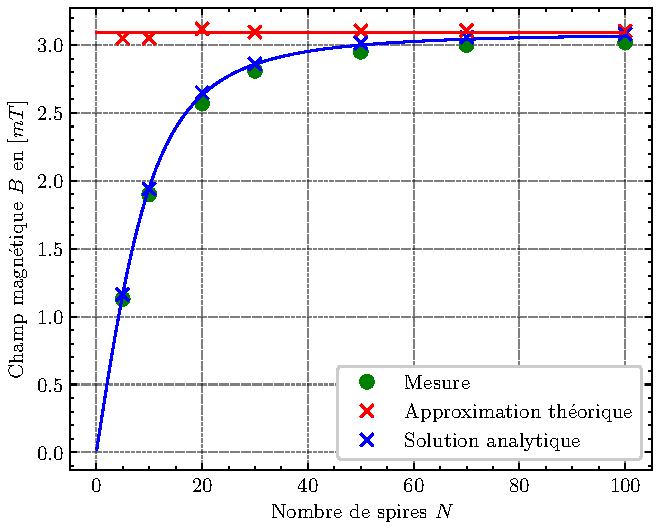
\includegraphics[width=.6\textwidth]{solenoide_1.pdf}

\caption{Comparaison entre la mesure et les différents modèles sur la première expérience}
\end{figure}

Afin de bien se rendre compte du moment dès lequel l'approximation par la loi d'Ampère du solénoïde parfait fonctionne, nous avons tracer l'erreur relative des deux modèles afin de les comparer.

\begin{figure}[H]
\centering
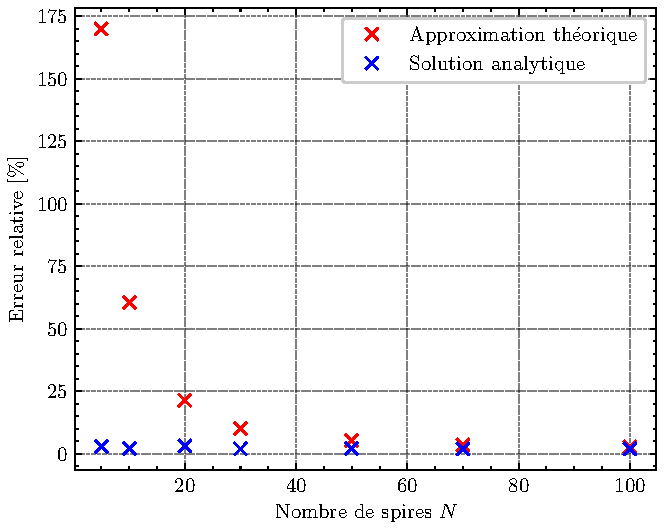
\includegraphics[width=.6\textwidth]{solenoide_2.pdf}

\caption{Erreur relative selon la taille du solénoïde}
\end{figure}

\paragraph*{Seconde expérience.} Les mesures de celle-ci se résument dans le décalage dénommé $x$ dans les équations, ainsi que le champs magnétique à cette position, ordonné selon le nombre de spire utilisé.\\ \\
Le calcul du champs de manière théorique est un peu plus compliqué, car il faut se rendre compte via de la trigonométrie élémentaire que $\tan \theta_{1,2} = \frac{r}{l \pm x}$. On obtient alors 
$$ B_{anal} = \frac{N I \mu_0}{l} \frac{\cos \left( \arctan \left( \frac{r}{l+x} \right) \right) + \cos \left( \arctan \left( \frac{r}{l-x} \right) \right)}{2} $$
pour lequel on utilise la valeur de l'arc tangente sur les quatre quadrants.\\ \\
Les différentes erreurs sont également consignées dans la table ci-dessous.

\begin{table}[H]
\centering
\resizebox{\textwidth}{!}{
\begin{tabular}{rrrrrrrrrrrrrrr}
\toprule
 \multicolumn{5}{l}{20 spires} & \multicolumn{5}{l}{50 spires} & \multicolumn{5}{l}{100 spires} \\
   décalage $[cm]$ &     $B \ [mT]$ & $B_{anal} \ [mT]$ &  $\Delta B_{anal} \ [mT]$ &  $\frac{\Delta B_{anal}}{B} \ [\%]$ &   décalage $[cm]$ &     $B \ [mT]$ & $B_{anal} \ [mT]$ &  $\Delta B_{anal} \ [mT]$ &  $\frac{\Delta B_{anal}}{B} \ [\%]$ &    décalage $[cm]$ &     $B \ [mT]$ & $B_{anal} \ [mT]$ &  $\Delta B_{anal} \ [mT]$ &  $\frac{\Delta B_{anal}}{B} \ [\%]$ \\
\midrule
    0.0 &  2.58 &        2.65 &           0.07 &            2.7 &    0.0 &  2.97 &       3.014 &          0.044 &           1.47 &     0.0 &  3.00 &       3.079 &          0.079 &           2.65 \\
    1.0 &  2.57 &       2.599 &          0.029 &           1.12 &    1.0 &  2.97 &       3.011 &          0.041 &           1.39 &     1.0 &  3.00 &       3.079 &          0.079 &           2.64 \\
    2.0 &  2.44 &       2.423 &          0.017 &            0.7 &    2.0 &  2.96 &       3.004 &          0.044 &           1.47 &     2.0 &  3.00 &       3.079 &          0.079 &           2.63 \\
    3.0 &  2.15 &       2.063 &          0.087 &           4.05 &    3.0 &  2.95 &       2.989 &          0.039 &           1.33 &     3.0 &  3.00 &       3.078 &          0.078 &           2.60 \\
    4.0 &  1.66 &       1.507 &          0.153 &            9.2 &    4.0 &  2.93 &       2.965 &          0.035 &            1.2 &     4.0 &  3.01 &       3.077 &          0.067 &           2.21 \\
    5.0 &  1.07 &       0.939 &          0.131 &          12.28 &    5.0 &   2.9 &       2.926 &          0.026 &            0.9 &     5.0 &  3.01 &       3.075 &          0.065 &           2.15 \\
    6.0 &  0.63 &       0.548 &          0.082 &          13.04 &    6.0 &  2.85 &       2.861 &          0.011 &           0.38 &     6.0 &  3.01 &       3.072 &          0.062 &           2.08 \\
    7.0 &  0.38 &       0.328 &          0.052 &          13.75 &    7.0 &  2.76 &       2.747 &          0.013 &           0.47 &     7.0 &  3.01 &       3.069 &          0.059 &           1.97 \\
    8.0 &  0.24 &       0.207 &          0.033 &          13.67 &    8.0 &  2.58 &       2.541 &          0.039 &           1.49 &     8.0 &  3.01 &       3.065 &          0.055 &           1.84 \\
    9.0 &  0.16 &       0.138 &          0.022 &          13.53 &    9.0 &  2.28 &       2.174 &          0.106 &           4.66 &     9.0 &  3.01 &       3.060 &          0.050 &           1.67 \\
   10.0 &  0.11 &       0.097 &          0.013 &          11.98 &   10.0 &   1.8 &       1.615 &          0.185 &          10.29 &    10.0 &  3.00 &       3.053 &          0.053 &           1.78 \\
   11.0 &  0.09 &        0.07 &           0.02 &          21.76 &   11.0 &   1.2 &       1.026 &          0.174 &           14.5 &    11.0 &  3.00 &       3.044 &          0.044 &           1.47 \\
   12.0 &  0.06 &       0.053 &          0.007 &          11.92 &   12.0 &  0.72 &       0.609 &          0.111 &          15.35 &    12.0 &  3.00 &       3.031 &          0.031 &           1.05 \\
   13.0 &  0.05 &       0.041 &          0.009 &          18.59 &   13.0 &  0.44 &       0.371 &          0.069 &          15.68 &    13.0 &  2.98 &       3.014 &          0.034 &           1.13 \\
   14.0 &  0.04 &       0.032 &          0.008 &          19.89 &   14.0 &   0.3 &       0.239 &          0.061 &          20.29 &    14.0 &  2.96 &       2.988 &          0.028 &           0.94 \\
   15.0 &  0.04 &       0.026 &          0.014 &          35.77 &   15.0 &  0.21 &       0.163 &          0.047 &          22.33 &    15.0 &  2.92 &       2.948 &          0.028 &           0.97 \\
   16.0 &  0.03 &       0.021 &          0.009 &          30.24 &   16.0 &  0.15 &       0.117 &          0.033 &          22.21 &    16.0 &  2.86 &       2.885 &          0.025 &           0.87 \\
   17.0 &  0.03 &       0.017 &          0.013 &           42.4 &   17.0 &  0.12 &       0.087 &          0.033 &          27.69 &    17.0 &  2.77 &       2.778 &          0.008 &           0.27 \\
   18.0 &  0.03 &       0.014 &          0.016 &          51.87 &   18.0 &   0.1 &       0.067 &          0.033 &          33.42 &    18.0 &  2.62 &       2.586 &          0.034 &           1.30 \\
   19.0 &  0.03 &       0.012 &          0.018 &          59.36 &   19.0 &  0.08 &       0.052 &          0.028 &          34.51 &    19.0 &  2.36 &       2.242 &          0.118 &           5.00 \\
   20.0 &  0.02 &        0.01 &           0.01 &          48.05 &   20.0 &  0.07 &       0.042 &          0.028 &          39.85 &    20.0 &  1.89 &       1.703 &          0.187 &           9.91 \\
        &       &             &                &                &   21.0 &  0.07 &       0.034 &          0.036 &           50.8 &    21.0 &  1.28 &       1.103 &          0.177 &          13.85 \\
        &       &             &                &                &   22.0 &  0.06 &       0.029 &          0.031 &          52.36 &    22.0 &  0.78 &       0.659 &          0.121 &          15.51 \\
        &       &             &                &                &   23.0 &  0.06 &       0.024 &          0.036 &          59.94 &    23.0 &  0.46 &       0.401 &          0.059 &          12.85 \\
        &       &             &                &                &        &       &             &                &                &    24.0 &  0.30 &       0.258 &          0.042 &          13.97 \\
        &       &             &                &                &        &       &             &                &                &    25.0 &  0.20 &       0.176 &          0.024 &          11.91 \\
        &       &             &                &                &        &       &             &                &                &    26.0 &  0.16 &       0.126 &          0.034 &          21.00 \\
\bottomrule
\end{tabular}}

\caption{Mesures et calcules de la seconde expérience}
\end{table}

Nous avons également comparés les mesures au modèle via des graphes. Celui en haut de la figure suivante correspond aux résultats liés aux 20 spires, celui du milieu aux 50 et le derniers aux 100.

\begin{figure}[H]
\centering
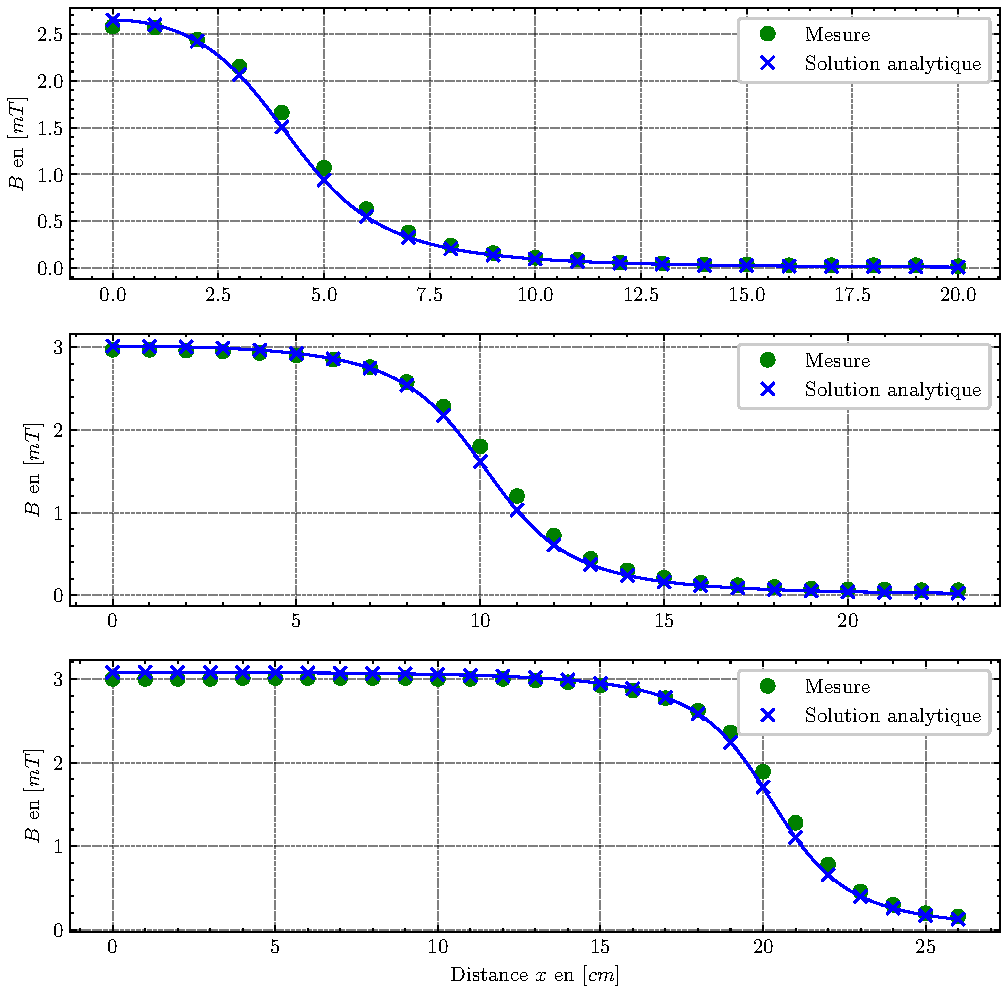
\includegraphics[width=.8\textwidth]{solenoide_3.pdf}

\caption{Comparaison entre les mesures et le modèle pour la seconde expérience}
\end{figure}